\section{Arbres de calcul (6 points)}

\begin{questions}
	\question[3] Décrire par une phrase les arbres de calcul suivant et écrire l'expression correspondante (le résultat n'est pas demandé).
	
	
	\begin{center}
		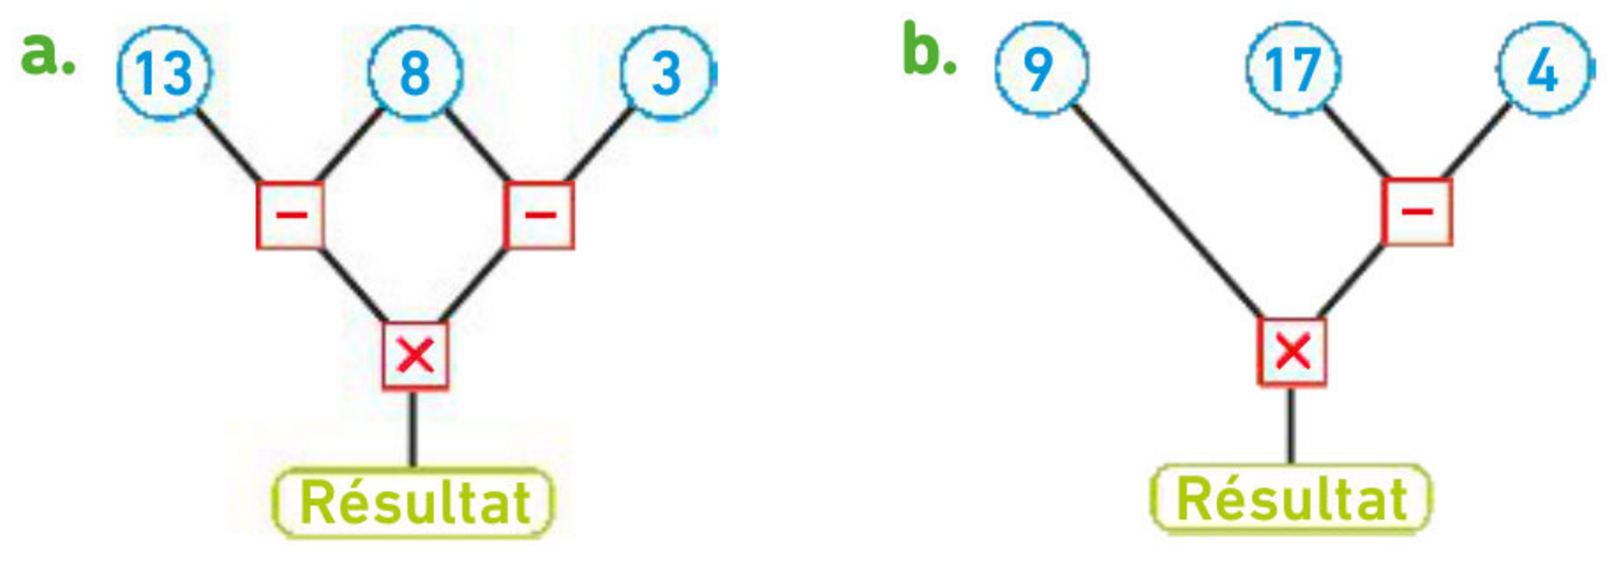
\includegraphics[scale=0.3]{img/arbres}
	\end{center}
	
	\question[3] Décrire par une phrase les expressions suivantes et dessiner l'arbre de calcul correspondant.
	
	\begin{multicols}{2}
		\begin{enumerate}
			\item $30 \times 4 + 20 \div 2$
			\item $30 \times (20 - 4)$
			%\item $10 + 4 \times 10$
		\end{enumerate}
	\end{multicols}	
\end{questions}
